\subsection[Restrições de Arquitetura]{Restrições de Arquitetura}

Esta seção fornece uma visão geral sobre as restrições propostas por Fielding para a implementação em elementos dentro de uma arquitetura de serviço web. Além disso, será examinado o impacto de cada restrição em sistemas distribuídos em hypermedia.

\textbf{Cliente-Servidor}

É a primeira restrição para uma aplicação REST.  Neste modelo, não existe conexão entre cliente e servidor, mas sim a espera do servidor por pedidos de clientes, executando solicitações e devolvendo uma resposta. Seu objetivo é separar arquitetura e responsabilidades dos ambientes cliente e servidor. Assim, o cliente (consumidor do serviço) não se preocupa com tarefas como a comunicação de banco de dados, gerenciamento de cache, etc. O inverso também é verdadeiro, onde o servidor (prestador de serviços) não está preocupado com as tarefas do cliente como interface, experiência do usuário etc. Assim, permitindo a evolução independente das duas arquiteturas desde que a interface de comunicação entre os dois não seja alterada. \cite{Fielding2000}

\textbf{Sem Estado}

Como HTTP é um protocolo sem conexão (onde não há nenhuma garantia sobre qual servidor será processado e quanto tempo irá levar) cada requisição deve conter todas as informações necessarias para que um servidor entenda o que um cliente está executando. Ou seja, para ser stateless, um servidor não pode guardar informações de estado do cliente, como sessões por exemplo. \cite{Fielding2000}

Esta restrição ajuda na viabilidade, confiabilidade e escalabilidade de sistemas distribuídos. Garantem que chamadas da API não estejam vinculadas a um determinado servidor. Contudo, com base no número da diversidade de clientes, ao manter um servidor sem estado é possível perder controle no tamanho de resposta, o que pode ser um fator crucial para aplicações que dependem disso. \cite{Wildermuth2015}

\textbf{Interface Uniforme}

Em essência, Fielding propõe que aplicações façam o uso de verbos HTTP (POST, GET, PUT, DELETE) e identificadores uniforme de recursos (URI) para mapear operações em ambientes distribuidos. Através de pequenas regras de acesso pelo cliente, é possível modificar/refatorar o servidor de maneira a minimizar riscos de acoplamento. Esta idéia, trouxe um pensamento diferente ao modelo RPC, cuja API dá ênfase a um maior número de operações. \cite{Fielding2000}

\begin{itemize}[noitemsep]
\item Identificação de Recursos: Cada recurso deve ter uma URI coesa e especifica para ser disponibilizado
\item Representação de Recurso: Formato de representação no qual um recurso vai ser retornado para um cliente. (Exemplo: HTML, XML, JSON, TXT)
\item Resposta Auto-explicativa: Uso de metadados na requisição e resposta. (Exemplo: código de resposta HTTP, Host, Content-Type)
\item HATEAOS\footnote{
  Hypermedia as the Engine of Application State.
} - Retornar na resposta hyperlinks para que o cliente saiba navegar em busca de mais recursos relacionados.
\end{itemize}

\textbf{Separação em Camadas}

Um dos principios desta restrição está em evitar que clientes façam diretamente requisição para o servidor sem antes passar por um intermediario, como um load balancer ou alguma alguma outra máquina que faça ponte entre servidores. Assegurando que clientes apenas se preocupem com a comunicação, deixando para que intermediários lidem com a distribuição de requisições. \cite{Fielding2000}

\begin{figure}[H]
  \centering
  \resizebox{\columnwidth}{!}{
    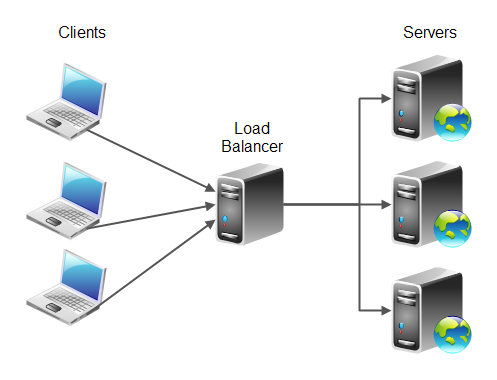
\includegraphics[width=\textwidth,height=\textheight,keepaspectratio]{figuras/load-balancer.png}
  }
  \caption{Exemplo de Load Balancer}
\end{figure}

\textbf{Código sob Demanda}

Apesar de ser a única restrição opcional do estilo, ela permite que servidores disponibilizem código em forma de script para que seja executado no cliente. Dessa forma, extendendo a lógica de serviço do servidor para seus clientes. \cite{Fielding2000}

\textbf{Cache}

Para aumentar desempenho de um serviço. Quando um recurso é acessado por mais de um cliente, se não houve mudança neste é recomendado que estas respostas sejam armazenadas em cache, evitando o processamento desnecessário. Isso significa que servidores, quando possível, devem implementar regras de cache para beneficio de ambos os ambientes. \cite{Fielding2000}
